%doc: Revista 3/PresentacioRB/presentacio.docx
\begin{news}
{2} %columnes
{Presentació del llibre: El documental com a estratègia educativa}
%index: El documental com a estratègia educativa
{El Ramon Breu, professor  de l’escola i company nostre, el dia 20 d’octubre va presentar el seu darrer llibre : EL DOCUMENTAL COMO ESTRATEGIA EDUCATIVA, a la Biblioteca plaça d'Europa}
{Fem Escola}
{250} %pagesof

\noindent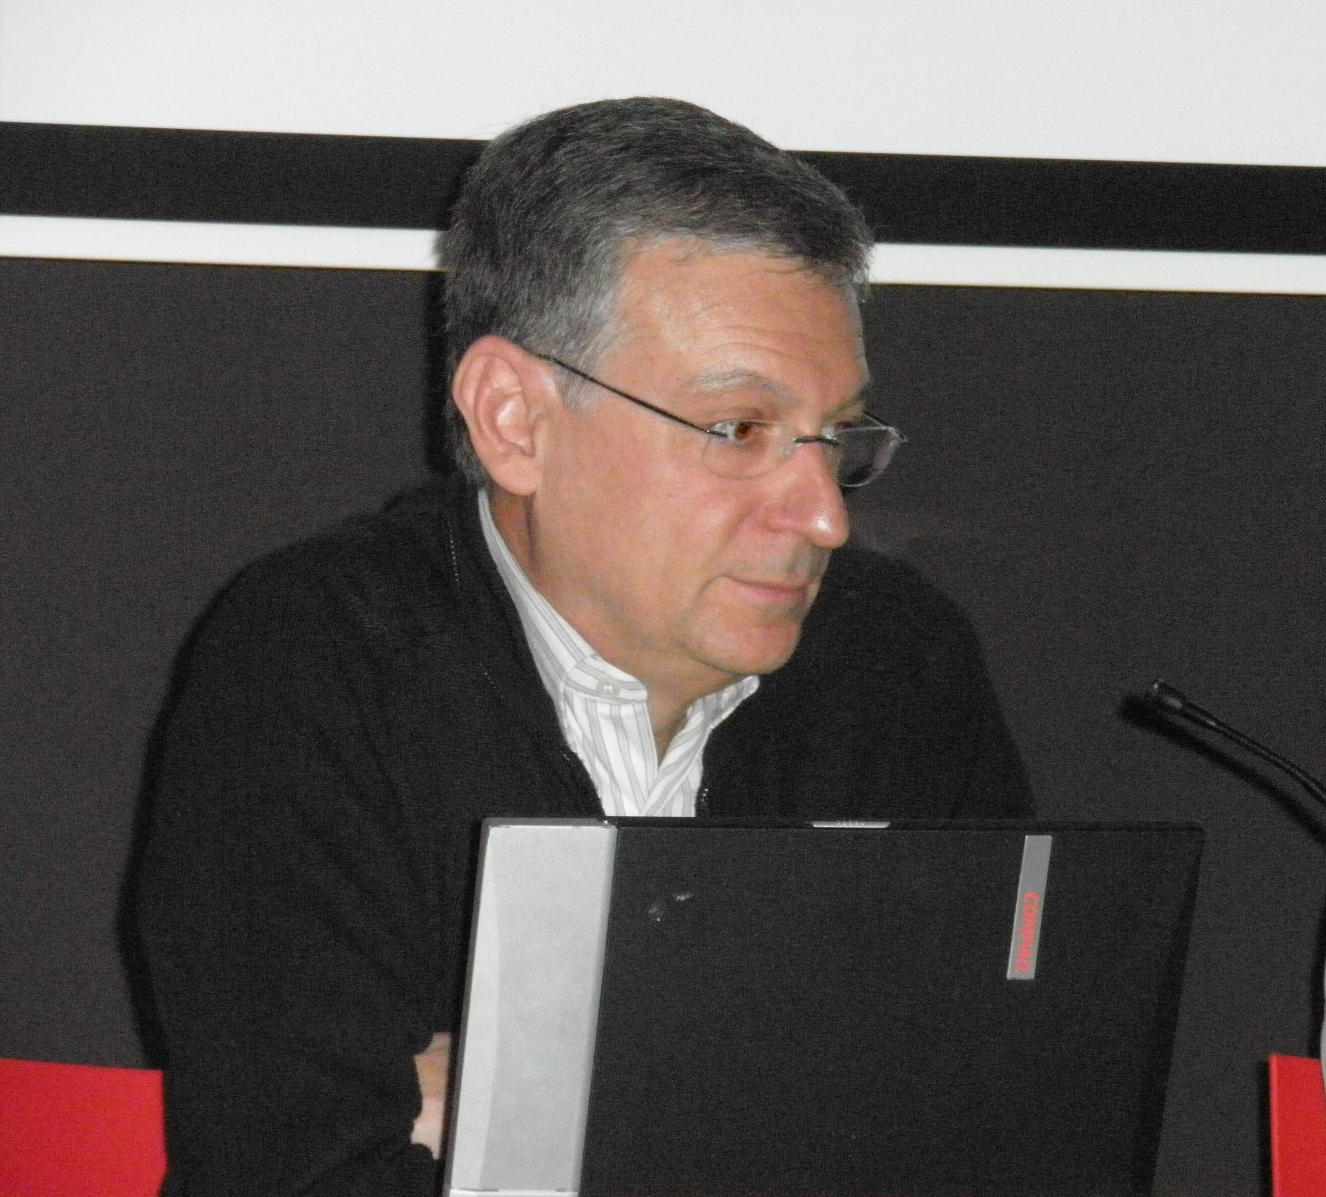
\includegraphics[width=9cm,keepaspectratio]{fem_escola/img/llibre_PA200015b.jpg}

%Amadeu Torner, 57 de l’Hospitalet de Llobregat.

Participaren de la presentació  David Urrea, director de la Biblioteca Plaça d'Europa, Cinta Vidal, directora d'Edicions de l'Editorial Graó i Alba Ambròs, professora de la Facultat d'Educació de la Universitat de Barcelona.

Va ser un acte entranyable i íntim;  en Ramon va estar molt ben acompanyat per la família, els companys, els  amics i per professionals diversos. 
A més, la biblioteca és un lloc molt significatiu i proper per en Ramon ja que està ubicada en  l’entorn on ell ha passat la infància i bona part de la seva vida.

Com a professionals de l’ensenyament valorem aquest llibre com una bona eina didàctica per a l’educació en valors i per a l’estudi i anàlisi del documental a les aules. Estem molt orgullosos de la il·lusió, dedicació i esperit de renovació que el nostre company és capaç d’aportar a l’ensenyament tot elaborant diferents materials didàctics i de reflexió que permeten millorar la qualitat pedagògica de les escoles. 

\authorandplace{Per molts anys, Ramón !}{}

\end{news}
